\documentclass{llncs}
\usepackage[pdfstartview={FitH}]{hyperref} 
\usepackage[ruled,vlined]{algorithm2e}
\usepackage{relsize}
\pagestyle{plain}
\toctitle
\tocauthor
\usepackage{etoolbox}
\usepackage{amsmath,amssymb,stmaryrd}
\usepackage{stmaryrd}
\usepackage{amssymb}
\usepackage{float}
\usepackage{cancel}
\DeclareMathOperator{\Pos}{Pos}
\def\regw#1{\Reg{(#1)}}
\DeclareMathOperator{\Reg}{RegExp}
\DeclareMathOperator{\Last}{Last}
\DeclareMathOperator{\last}{Fl_0} 
\DeclareMathOperator{\Follw}{Fl_>}
\DeclareMathOperator{\First}{First}
\DeclareMathOperator{\Follow}{Follow}
\DeclareMathOperator{\Leave}{Leaves}
\DeclareMathOperator{\RegE}{RegExp}
\DeclareMathOperator{\regTree}{RegTreeExp}
\DeclareMathOperator{\E}{E}
\DeclareMathOperator{\oo}{O}
\DeclareMathOperator{\h}{H}
\DeclareMathOperator{\f}{F}
\DeclareMathOperator{\ar}{R}
\DeclareMathOperator{\G}{G}
\DeclareMathOperator{\Fir}{Fr_>}
\DeclareMathOperator{\Firs}{Fr_0}
\def\PO#1#2{Pos_{0#1}{\left(#2\right)}}
\def\b#1{\overline{#1}}
\usepackage{pgf}
\usepackage{tikz}
\usepackage{tikz}
\usetikzlibrary{automata}
\usetikzlibrary{shadows}
\usetikzlibrary{arrows}
\usetikzlibrary{shapes}
\usetikzlibrary{decorations.pathmorphing}
\usetikzlibrary{fit}
\tikzstyle{every picture}=[>=stealth',shorten >=1pt,node distance=1.44cm,bend angle=45,initial text=,every state/.style={inner sep=0.75mm, minimum size=1mm},font=\scriptsize]
\addtolength{\intextsep}{-7mm}
\usepackage{theorem}
\usepackage{stmaryrd}
\usepackage{amsxtra}
\usepackage{amssymb}
\usepackage{graphicx}
\DeclareMathOperator{\rooot}{root}
\def\first#1{\First{(#1)}}
\def\Po#1#2{\Pos_{#1}{(#2)}}
\def\firstt#1{\Fir{(#1)}}
\def\firs#1{\Firs{(#1)}}
\def\Fl#1#2{\Follow{(#1,#2)}}
\def\Fll#1#2#3{\Follow{(#1,#2,#3)}}
\def\Flw#1#2{\Folw{(#1,#2)}}
 \def\las#1#2#3{\last{(#1,#2,#3)}}
\def\Fw#1#2#3{\Follw{(#1,#2,#3)}}
\def\lst#1#2{\la{(#1,#2)}}
\def\regt#1{\regTree{(#1)}}
\title{Algorithm for the -Position Tree Automaton Construction\thanks{D. Ziadi was supported by the MESRS - Algeria under Project 8/U03/7015.}} 
\author{Nadia Ouali Sebti \and Djelloul Ziadi \thanks{\email{Nadia.Ouali-Sebti, Djelloul.Ziadi@univ-rouen.fr}}}
\institute{Laboratoire LITIS - EA 4108 Universit\'e de Rouen, Avenue de l'Universit\'e \\76801 Saint-\'Etienne-du-Rouvray Cedex.} 
\authorrunning{N. Ouali Sebti, D. Ziadi}
\date{}
\begin{document}
\setcounter{footnote}{0}
\maketitle             
\begin{abstract}
The word position automaton was introduced by Glushkov and McNaughton in the early . This automaton
is homogeneous and has  states for a word expression of alphabetic width .
This kind of automata is extended to regular tree expressions.

In this paper, we give an efficient algorithm that computes the  sets, which are used in different algorithms of conversion of a regular expression into tree automata. In the following, we consider the -position tree automaton construction. We prove that for a regular expression  of a size  and alphabetic width , the  sets can be computed in  time complexity.   
\end{abstract}
\section{Introduction}

This paper is an extended version of ~\cite{Ouali}.

Regular expressions, which are finite representatives of potentially infinite languages, are widely used in various application areas such as XML Schema Languages~\cite{xml}, logic and verification, \emph{etc.} The concept of word regular expressions  has been extended to tree regular expressions. 


 In the case of words, it is agreed that each regular expression can be transformed into a non-deterministic finite automaton.
Computer scientists have been interested in designing efficient algorithms for the computation of the position automaton. 
Three well-known algorithms for the computation of this automaton exist. The first makes use 
of the notion of star normal form ~\cite{Brug} of a regular expression   . The second is based on a
lazy computation technique ~\cite{Paig}. The third is built on the so-called ZPC-structure ~\cite{ZPC}.
The complexity of these three algorithms is quadratic with regard to the size of the regular expression.


This study is motivated by the development of a library of functions for handling rational kernels ~\cite{mohri1} in the case of trees. The first problem consists of the conversion of a regular expression into a tree automaton. 

Recently Kuske and Meinecke~\cite{automate2} proposed an Algorithm to construct an equation automaton~\cite{antimirov,ouardi} from a regular tree expression    with an  time complexity where  is the size of  and  is the maximal rank appearing in the ranked alphabet. 
This algorithm is an adaptation to trees of the one given by Champarnaud and Ziadi in the case of words~\cite{ZPC}. 
This generalization is interesting although the adaptation of the word algorithm to trees is not obvious at all.
Indeed, the Champarnaud and Ziadi Algorithm, for the construction of the set of transitions, is based 
on the computation of some function called "" which is not yet defined on trees.  
Notice that the star normal form of a regular tree expression  can not be defined, this notion doesn't make sense.  
For these reasons the definition of the  function in the case of trees is given in this paper, while an efficient algorithm for its computation (computation of the -position tree automaton) is proposed. 

The paper is organized as follows: Section~\ref{sec prelim} outlines finite tree automata over ranked alphabets, regular tree expressions, and linearized regular tree expressions. Next, in Section~\ref{sec automata} the notions of  and  of regular expressions and the -position automaton are recalled. Then, in Section~\ref{sec algo} we present an efficient algorithm which builds the -position tree automaton with an  time complexity. Finally, the different results described in this paper are given in the conclusion. 

\section{Preliminaries}\label{sec prelim}
    Let  be  \emph{a ranked alphabet}, where  is a finite set and  represents the  \emph{rank} of  which is a mapping from  into . The set of symbols of rank  is denoted by . The elements of rank  are called  \emph{constants}. A \emph{tree}  over    is inductively defined as follows:  where  is any symbol in  ,  is any integer satisfying ,  is any symbol in  and  are any  trees over . We denote by  the set of trees over .  \emph{A tree language} is a subset of . Let  denote the set of  \emph{non-constant symbols} of the ranked alphabet . \emph{A Finite Tree Automaton} (FTA)~~\cite{automate1,automate2}  is a tuple  where  is a finite set of states,  is the set of \emph{final states} 
and   is the set of  \emph{transition rules}. This set is equivalent to the function  from  to  defined  by . The domain of this function can be extended to 
as follows: .  Finally, we denote by  the function from    defined for any tree in  as follows: 
   if   with , 
   if  with  and . 
  A tree is \emph{accepted} by  if and only if .   
 
  The language  \emph{recognized} by  is the set of trees accepted by   \emph{i.e.} . 

For any integer , for any  languages , and for any symbol  ,  is the tree language . The \emph{tree substitution} of a constant  in  by a language  in a tree , denoted by , is the language inductively defined by:
    if ;  if  where ;  if  with  and  any  trees over .   
    Let  be a symbol in . The -\emph{product}  of two languages  is  defined by . The \emph{iterated -product} is  inductively  defined for  by:   and . The -\emph{closure} of  is defined by  .
    
A \emph{regular expression } over a ranked alphabet  is inductively defined by  , , , , , , where , ,  and  are any  regular expression s over . Parenthesis can be omitted when there is no ambiguity. We write  if  and  graphically coincide. We denote by  the set of all regular expression s over . Every regular expression   can be seen as a tree over the ranked alphabet  where  and  can be seen as symbols
 of rank  and  has rank . This tree is the syntax-tree  of . We denote by  the number of occurrences of a symbol  in a regular expression . The \emph{alphabetic width}  of  is the number of occurrences of symbols of  in  ( ). \emph{The size}  of  is the size of its syntax tree . The \emph{language}   \emph{denoted by}  is inductively defined by
 , , , , ,  where  ,  are any  regular expression s,   and . It is well known that a tree language  is accepted by some tree automaton if and only if it can be denoted by a regular expression  ~\cite{automate1,automate2}.
A regular expression   defined over  is  \emph{linear} 
if every symbol of rank greater than  appears at most once in . Note that any constant symbol may occur more than once. Let  be a regular expression  over . The  \emph{linearized regular expression }  in  of a regular expression   is obtained from  by marking differently all symbols of a rank  greater than or equal to  (symbols of ). The marked symbols form together with the constants in  a ranked alphabet  the symbols of which we call \emph{positions}.
The mapping  is defined from  to  with  for every  . It associates with a marked symbol  the symbol  and for a symbol  the symbol .
We can extend the mapping  naturally to   by , , , , , with , , ,  such that  and  any regular expression s over . 


\section{The -Position Tree Automaton}\label{sec automata}

The set of positions associated to  are straightforwardly deduced from the set of symbols associated to . 
In order to construct a nondeterministic finite automaton (position tree automaton) associated to the 
regular expression   that recognizes ,
we need to define two sets, the set  and the set  for a position .


  In the following of this section,  is a regular expression  over a ranked alphabet . 
  The set of symbols in  that appear in an expression  is denoted by .


  In this section, we show how to compute the -position tree automaton of a regular expression   , recognizing . This is an extension of the well-known position automaton~~\cite{glushkov} for word regular expression  s where the  represents the fact that any -ary symbol is no longer a state of the automaton, but is exploded into  states.
  The same method was presented independently by McNaughton and Yamada~~\cite{mcnaughton60}.  
   Its computation is based on the computations of particular \emph{position functions}, defined in the following.
  
  In what follows, for any two trees  and , we denote by  the relation " is a subtree of ".
  Let  be a tree. 
We denote by  the root of , by  the  child of  in , that is the root of  if it exists, and by  the set of the leaves of , \emph{i.e.} . 
  We denote by  the root of , by  the  child of  in , that is the root of  if it exists, and by  the set of the leaves of , \emph{i.e.} . 
  
  Let  be a regular expression  and  its linearized form,  be two integers and  be a symbol in  and  be a position in  with .

  The set  is the subset of  defined by ; The set  is the subset of  defined by ; The set  is the subset of  defined by .
  
 \begin{example}\label{Pos Automat}
 Let  be defined by ,  and .
    Let us consider the regular expression    and its linearized form defined by:
   
    
\noindent,
   
    
\noindent.
      
The language denoted by  is .

Consequently,  and , , , , ,  . 
\end{example}  
 

The two functions  and  are sufficient to construct the \emph{-position tree automaton} from a regular expression  . 
 
  \begin{definition}\label{def aut pos}~\cite{arxiv}
    Let  be a regular expression ,  and  be symbols in  and  and  be positions in  with  and . The -\emph{Position Tree Automaton}  is the automaton  defined by 
       
\centerline{}       
       
      
  \end{definition}
  
  It has been shown in ~\cite{arxiv} that the -position tree automaton of  accepts , hence the following theorem:   

  
    \begin{theorem}\label{thm lang pe eq e}~\cite{arxiv}
     Let  be a regular expression, then .
  \end{theorem}
    
\begin{example}
The -Position Automaton  associated with  of Example~\ref{Pos Automat} is given in Figure~\ref{fig a t e2}.
The set of states is . The set of final states is . 
The set of transition rules  is 

\centerline{
    , , ,
}

\centerline{
    , , ,
}

\centerline{
    , ,
}

\centerline{
    , , , ,
}

\centerline{
    , , , ,
}

\centerline{
   , , , , , , 
}

The -Position Automaton  associated with  is represented in Figure~\ref{fig a t e2}.
\end{example}

\begin{figure}[H]
  \centerline{
	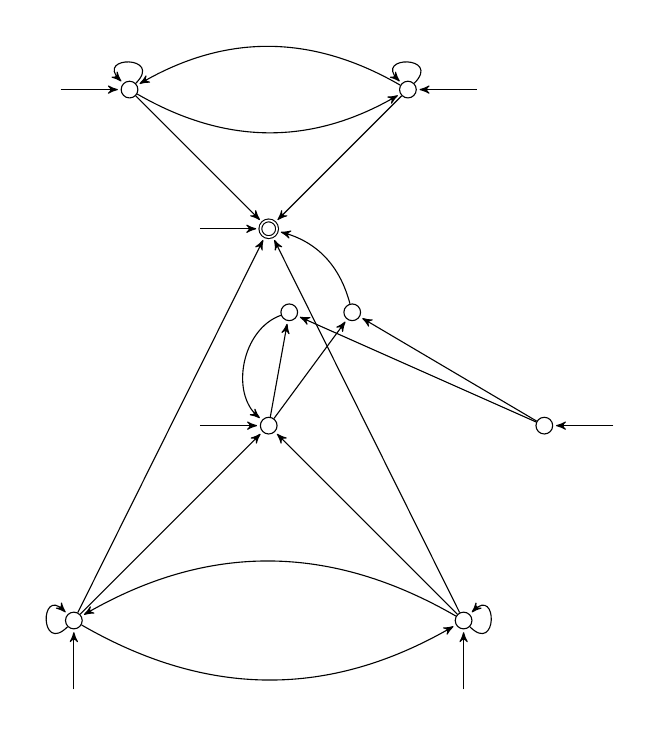
\begin{tikzpicture}[node distance=2.5cm,bend angle=30,transform shape,scale=1]
\node[accepting,state] (eps) {};
	  \node[state, above left of=eps] (f11) {};	
	  \node[state, above right of=eps] (h12) {}; 
      \node[state, below of=eps] (g13) {};
      \node[state, below right of=eps,node distance=1.5cm] (cer1) {};
      \node[state, left of=cer1,node distance=0.8cm] (cer) {};
      \node[state, right of=g13,node distance=3.5cm] (g23) {};
	  \node[state, below left of=g13,node distance=3.5cm] (h15) {};
      \node[state, below right of=g13,node distance=3.5cm] (f14) {};
\draw (eps) ++(-1cm,0cm) node {}  edge[->] (eps);  
	  \draw (f11) ++(-1cm,0cm) node {}  edge[->] (f11);  
	  \draw (h12) ++(1cm,0cm) node {}  edge[->] (h12); 
	  \draw (h15) ++(0cm,-1cm) node {}  edge[->] (h15);  
	  \draw (g23) ++(1cm,0cm) node {}  edge[->] (g23);  
	  \draw (g13) ++(-1cm,0cm) node {}  edge[->] (g13);    
	  \draw (f14) ++(0cm,-1cm) node {}  edge[->] (f14);
\path[->]
        (f11) edge[->,below left] node {} (eps)
		(f11) edge[->,loop,above] node {} ()
		(h12) edge[->,bend right,above] node {} (f11)
		(g13) edge[->] node {} (cer1)
		(g23) edge[->] node {} (cer1)	
		(cer1) edge[->,bend right,above right] node {} (eps)
		(g13) edge[->] node {} (cer)
		(g23) edge[->] node {} (cer)	
		(cer) edge[->,bend right=60,above right] node {} (g13)		  
		(h12) edge[->,loop,above] node {} ()
		(h12) edge[->,below right] node {} (eps)
		(f11) edge[->,bend right,above] node {} (h12)
		(h15) edge[->, in=135,out=-135,loop,left] node {} ()	
		(h15) edge[->,above left] node {} (eps)		
		(h15) edge[->,above left] node {} (g13)		
		(h15) edge[->,bend right,above] node {} (f14)
		(f14) edge[->,in=45,out=-45,loop,right] node {} ()	
		(f14) edge[->,bend right,above] node {} (h15)		
		(f14) edge[->,above right] node {} (eps)		
		(f14) edge[->,above right] node {} (g13)
	  ;
      \end{tikzpicture}
  }
  \caption{The -Position Automaton  of .}
  \label{fig a t e2}
\end{figure}	

In the following sections, we will show how we can efficiently compute the function . This algorithm can be used in different constructions such us the equation automaton~\cite{automate2}, \emph{-C-continuation automaton}~\cite{cie,arxiv} and Follow Automaton~\cite{arxiv}.

\section{Efficient computation of the function }\label{sec algo}
In ~\cite{automate1} Champarnaud and Ziadi gave in the case of words an algorithm with an  space and time complexity. 
They enhanced the algorithm to one with an  time and space complexity.
In ~\cite{automate2}, Kuske and Meinecke extend the algorithm based on the notion of word partial derivatives ~\cite{antimirov} to tree partial derivatives in order to compute from a regular expression    a tree automaton recognizing . Laugerotte et al. proposed an algorithm for the computation of the position tree automaton and the reduced tree automaton in~\cite{Ouali}. This is an extended version of ~\cite{Ouali}. In~\cite{cie,arxiv2} Mignot et al. gave an efficient algorithm for the computation of the equation automaton using the -c-continuations. 


In this section we will describe an algorithm for the computation of the -position tree automaton based on the computation of the  function.


In the following, we will inductively replace each regular subexpression  of  by the regular subexpression . The regular expressions considered thereafter are already dealt by this transformation.

 
By misuse of language we will denote by  for  and by  for . Let us first show that the functions  and  can be inductively computed.
 
  \begin{lemma}\label{firstComput}~\cite{arxiv}
     Let  be a linear regular expression.  
    The set  can be computed as follows:
    
    \centerline{, ,}
    
\centerline{ , 
}    
    
    \centerline{,}
    
     \centerline{,}
    
    \centerline{
      
    }
  \end{lemma}  
  
  \begin{lemma}\label{Computfollow}~\cite{arxiv}
   Let  be a linear regular expression,  be two integers and  be a symbol in . 
  
    The set of symbols  can be computed inductively as follows:
    
    \centerline{,}
    
    \centerline{
      
    }
    
    \centerline{
      
    }
    
    \centerline{
      
    }
    
    \centerline{
      
    }
  \end{lemma} 
The main idea of our algorithm consists of the separation of the computation of the function  (resp. ) to the computation of two subsets  (resp. ) and  (resp. ) that are respectively  
the projection of the set  (resp. ) to the positions associated with
symbols of a rank  and a rank greater than .

Thus the computation of the set  can be written as follows:  
 


\begin{proposition}
 \label{s}
Let  be a linear regular expression and  be a subexpression of . The set of symbols  is defined as follows:

\end{proposition}
\begin{proof}
\begin{sloppy}  
  
Let  be a linear regular expression,  be two integers and  be a symbol in .
\begin{enumerate}
\item If  or if , then  and for , .  

\item Let us prove this proposition for the case . 

We have 
 
\end{enumerate}
\end{sloppy}  
  \qed
\end{proof} 
The following proposition shows that  can be computed in a similar way to the case of words. 
\begin{proposition}
\label{prop firstsup}
Let  be a linear regular expression and  be a subexpression of . The set of symbols  is defined as: 

\end{proposition}
\begin{proof}
\begin{sloppy}  
  
Let  be a linear regular expression. 
\begin{enumerate}
\item If  or if , then  and for , .  

\item Let us prove this proposition for the cases . 

We have 
 
\end{enumerate}
\end{sloppy}  
\qed
\end{proof}

Let us recall that  and  are, respectively, the projection of the set  to the symbols associated with symbols of a rank  and a rank greater than . We have: 

\begin{proposition}\label{a}
Let  be a linear regular expression,  be two integers and  be a symbol in . 
The function  can be computed inductively as follows: 

\end{proposition}


\begin{proof}
\begin{sloppy}  
  
Let  be a linear regular expression,  be two integers and  be a symbol in .  
\begin{enumerate}
\item If  or if , then .

Let us prove this proposition for the cases  and . 
\item Let us consider that . 

We have 

\item Let us consider that . By definition we have . Then: 
 
\end{enumerate}
\end{sloppy}   
\qed
\end{proof}

\begin{proposition}
\label{x}
Let  be a linear regular expression,  be two integers and  be a symbol in .  
We define inductively the set  as follows:

\end{proposition}
\begin{proof}
\begin{sloppy}  
  
Let  be a linear regular expression,  be two integers and  be a symbol in . 
\begin{enumerate}
\item If  or if , then .\\
Let us prove this proposition for the cases  and . 
\item Let us consider that . 

We have 

\item Let us consider that . By definition we have . Then: 
 
\end{enumerate}
\end{sloppy}    
\qed
\end{proof}
\begin{remark}\label{remark}
The definition of the set  is identical to the function  in the case of words~\cite{ZPC}. We have the same formulas.
\end{remark} 



The construction of the -position tree automaton  from the regular expression  as it has been presented in this article complies with the properties of the position automaton proposed by Glushkov. 
This is the generalization of the position automaton from words to trees.

\subsection{-Structure for  Computation}
In the word case, the construction of the position automaton, has been developed in~\cite{ZPC96,ZPC}. This construction will be extended to trees in the following.
 
Let  be the syntax tree associated with the regular expression  . 

The set of nodes of  is written as . For a node  in , , , ,  and  denote respectively the symbol, the father, the son, the right son and the left son of the node  if they exist. 

We denote by  the subexpression rooted at ; In this case we write  to denote the node associated to . Let  be the function defined by: 

 
    
    

\noindent where  is an artificial node such that . The -Structure is the syntax tree equipped with  links.

We extend the relation  to the set of nodes of : For two nodes  and  we write . We define the set  which is totally ordered by .


\begin{proposition}\label{b}
Let  be linear regular expression,  be two integers and  be in . Then  where  is the node of  labelled by ,  is the ,  and for  such that .
\end{proposition}
\begin{proof}
\begin{sloppy}
  By induction over the structure of .
  \begin{enumerate}
    \item Let us suppose that . Then . Since by definition  is the root of ,  is the root of . Hence .
    \item Let us suppose that  with , or , or  with . Then  with . By induction hypothesis,  where  is the node of  labelled by ,  is the ,  and for  such that . Since ,  where  is the node of  labelled by ,  is the ,  and for  such that 
.    
    \item Let us suppose that  with  (resp. ). Then  with . By induction hypothesis,  where  is the node of  labelled by ,  is the ,  and for  such that . 
    
    Since , by setting  and ,  where  is the node of  labelled by ,  is the ,  and for  such that .
  \end{enumerate}
\end{sloppy}  
  \qed
\end{proof}

\subsection{Description of the algorithm and complexity}

An implicit construction of the word position automaton, the so-called ZPC-structure, has been developed by Ziadi et al. \cite{ZPC96,ZPC}.
Algorithm~\ref{zpc} extends this construction to the regular tree expressions. It constructs
a forest of trees where every tree rooted at a node  represents the set  according to Proposition~\ref{prop firstsup}. 

\begin{algorithm}[H]
\caption{-Structure Construction}
\label{zpc}
\KwIn{Regular Expression .}
\KwOut{-Structure}
 Construct the syntax tree   of ;\\
{\#}\\
\For{each node  on }{
	 Compute \;
\textbf{end for}  }
{\# The construction of a  Forest}\\
\For{each node  in }{
	\If{}{
 		 Remove the link \;
	\textbf{end if}}
\textbf{end for}}
{\# We have }\\
\For{each node  in }{
	\For{ to }{
 		 Remove the link \;
		\textbf{end for}}
\textbf{end for}}
\For{each node }{
Delete the node \; 
\textbf{end for}}
{\# }\\
{\# The construction of  links ( links)}\\
 \For{each node  in }{
  create a follow link from  to \;
  \textbf{end for}}
 \For{each node  in }{
  create a link from  to \;
  \textbf{end for} }
  {\ }\\
     \Return{-Structure}
\end{algorithm}
\begin{example}
The syntax tree   associated with the regular expression   is given in Figure~\ref{fig a t e}. 
	\end{example}

\begin{figure}[H] 
	 \centerline{
	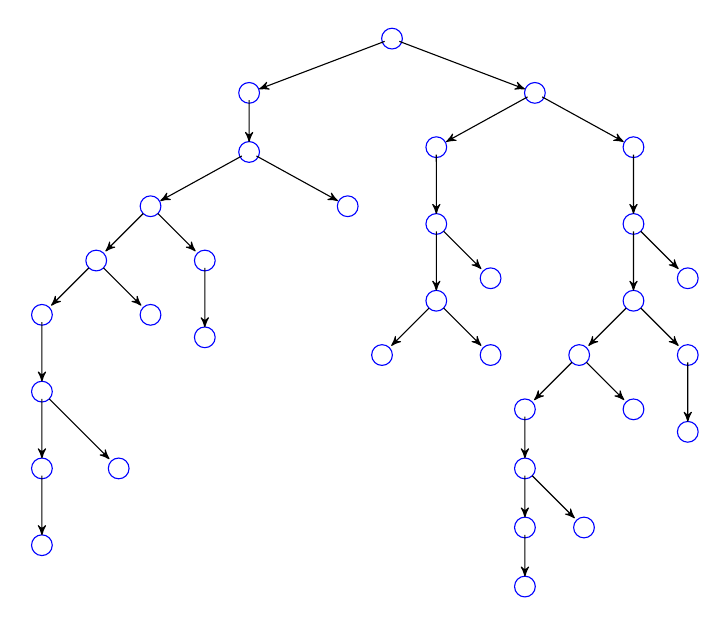
\begin{tikzpicture}[node distance=1.3cm,bend angle=30,transform shape,scale=.75]
		\node(1) {};		
		\node[below right of=1,xshift=1.5cm] (3) {};
		\node[below left of=1,xshift=-1.5cm] (22) {};			
		\node[below of=22,node distance=1cm] (221) {};		
		\node[below left of=221,xshift=-.75cm] (5) {};	 
		\node[below right of=221,xshift=.75cm] (222) {};  
		\node[below right of=5] (16) {};		 
		\node[below of=16] (4) {};
		\node[below left of=5] (17) {};
		\node[below left of=17] (18) {}; 
	 \node[below right of=17] (19) {};
	  \node[below of=18] (181) {};
	   \node[below of=181] (182) {};
	   \node[right of=182] (184) {};
	   \node[below of=182] (183) {};
		\node[below right of=3,xshift=.75cm] (6) {};
		\node[below of=6] (61) {};
        \node[below right of=61] (62) {}; 
		\node[below of=61] (51) {};
		\node[below right of=51] (116) {};		 
		\node[below of=116] (41) {};
		\node[below left of=51] (117) {};
		\node[below left of=117] (118) {}; 
	 \node[below right of=117] (119) {};
	  \node[node distance=1cm,below of=118] (1181) {};
	   \node[node distance=1cm,below of=1181] (1182) {};
	  \node[node distance=1cm,below of=1182] (1183) {};
	  \node[node distance=1cm,right of=1182] (1184) {};
	\node[below left of=3,xshift=-.75cm] (31) {};	
	\node[below of=31] (3121) {};
	\node[below of=3121] (312) {};
	\node[below right of=3121] (3122) {};	 
	\node[below right of=312] (311) {};
	\node[below left of=312] (313) {};
	\node[inner sep=0pt,draw, circle, fit=(1183), color=blue] (eqa1) {};
	\node[inner sep=0pt,draw, circle, fit=(1184), color=blue] (eqa1) {};
	   \node[inner sep=0pt,draw, circle, fit=(51), color=blue] (eqa1) {};
	   \node[inner sep=0pt,draw, circle, fit=(116), color=blue] (eqa1) {};
	   \node[inner sep=0pt,draw, circle, fit=(41), color=blue] (eqa1) {};
	   \node[inner sep=0pt,draw, circle, fit=(117), color=blue] (eqa1) {};
	   \node[inner sep=0pt,draw, circle, fit=(118), color=blue] (eqa1) {};	   
	   \node[inner sep=0pt,draw, circle, fit=(119), color=blue] (eqa1) {};
	   \node[inner sep=0pt,draw, circle, fit=(1181), color=blue] (eqa1) {};
	   \node[inner sep=0pt,draw, circle, fit=(1182), color=blue] (eqa1) {};
	 \node[inner sep=0pt,draw, circle, fit=(1), color=blue] (eq1) {};
\node[inner sep=0pt,draw, circle, fit=(181), color=blue] (eqf1) {};
\node[inner sep=0pt,draw, circle, fit=(182), color=blue] (eqa1) {};		
\node[inner sep=0pt,draw, circle, fit=(183), color=blue] (eqa1) {};	
\node[inner sep=0pt,draw, circle, fit=(184), color=blue] (eqa1) {};
	    \node[inner sep=0pt,draw, circle, fit=(22), color=blue] (eq2) {};	    
	    \node[inner sep=0pt,draw, circle, fit=(221), color=blue] (eq2) {};   
	    \node[inner sep=0pt,draw, circle, fit=(222), color=blue] (eq2) {};
	    \node[inner sep=0pt,draw, circle, fit=(3), color=blue] (eq3) {};
	    \node[inner sep=0pt,draw, circle, fit=(5), color=blue] (eq4) {};
	    \node[inner sep=0pt,draw, circle, fit=(4), color=blue] (eq5) {};
	    \node[inner sep=0pt,draw, circle, fit=(16), color=blue] (eq6) {};
	    \node[inner sep=0pt,draw, circle, fit=(19), color=blue] (eq7) {};
	    \node[inner sep=0pt,draw, circle, fit=(18), color=blue] (eq8) {};	
	    \node[inner sep=0pt,draw, circle, fit=(17), color=blue] (eq9) {};
	    \node[inner sep=0pt,draw, circle, fit=(62), color=blue] (eq10) {};  
	    \node[inner sep=0pt,draw, circle, fit=(61), color=blue] (eq10) {};    
	    \node[inner sep=0pt,draw, circle, fit=(6), color=blue] (eq10) {};
	   \node[inner sep=0pt,draw, circle, fit=(311), color=blue] (eq11) {};
	    \node[inner sep=0pt,draw, circle, fit=(313), color=blue] (eq121) {};
	   \node[inner sep=0pt,draw, circle, fit=(3121), color=blue] (eq12) {};
	   \node[inner sep=0pt,draw, circle, fit=(312), color=blue] (eq12) {};
	   \node[inner sep=0pt,draw, circle, fit=(3122), color=blue] (eq12) {};
	   \node[inner sep=0pt,draw, circle, fit=(31), color=blue] (eq13) {};
	 \path[->]
	 (18) edge node[above left,pos=0.4] {} (181)
	 (181) edge node[above left,pos=0.4] {} (182)
	 (182) edge node[above left,pos=0.4] {} (183)
	 (181) edge node[above left,pos=0.4] {} (184)
	      (1) edge node[above left,pos=0.4] {} (22)
	      (1) edge node[above right,pos=0.4] {} (3)
	      (16) edge node[left,pos=0.4] {} (4)
	      (61) edge node[left,pos=0.4] {} (62)
	      (6) edge node[left,pos=0.4] {} (61)
	      (61) edge node[left,pos=0.4] {} (51)
	      (22) edge node[left,pos=0.4] {} (221)
	      (221) edge node[left,pos=0.4] {} (222)
	      (221) edge node[left,pos=0.4] {} (5)
	      (3) edge node[right,pos=0.4] {} (6)
	      (5) edge node[above left,pos=0.4] {} (16)
	      (5) edge node[above left,pos=0.4] {} (17)
	      (17) edge node[left,pos=0.4] {} (18)
	      (17) edge node[left,pos=0.4] {} (19)
	      (3) edge node[left,pos=0.4] {} (31)
	      (31) edge node[left,pos=0.4] {} (3121)
	      (3121) edge node[left,pos=0.4] {} (3122)
	      (3121) edge node[left,pos=0.4] {} (312)
	      (312) edge node[left,pos=0.4] {} (311)
	      (312) edge node[left,pos=0.4] {} (313)
	      (51) edge node[left,pos=0.4] {} (116)
	      (116) edge node[left,pos=0.4] {} (41)
	      (51) edge node[left,pos=0.4] {} (117)
	      (117)edge node[left,pos=0.4] {} (118)
	      (117)edge node[left,pos=0.4] {} (119)
	      (118)edge node[left,pos=0.4] {} (1181)(1181)edge node[left,pos=0.4] {} (1184)
	      (1181)edge node[left,pos=0.4] {} (1182)(1182)edge node[left,pos=0.4] {} (1183)
	     ;
	     \end{tikzpicture}
	 }
\caption{The syntax tree   of }
	 \label{fig a t e}
	\end{figure}
	
 The -Structure associated with  is given in Figure~\ref{fig zpc e}.
\begin{figure}[H] 
	 \centerline{
	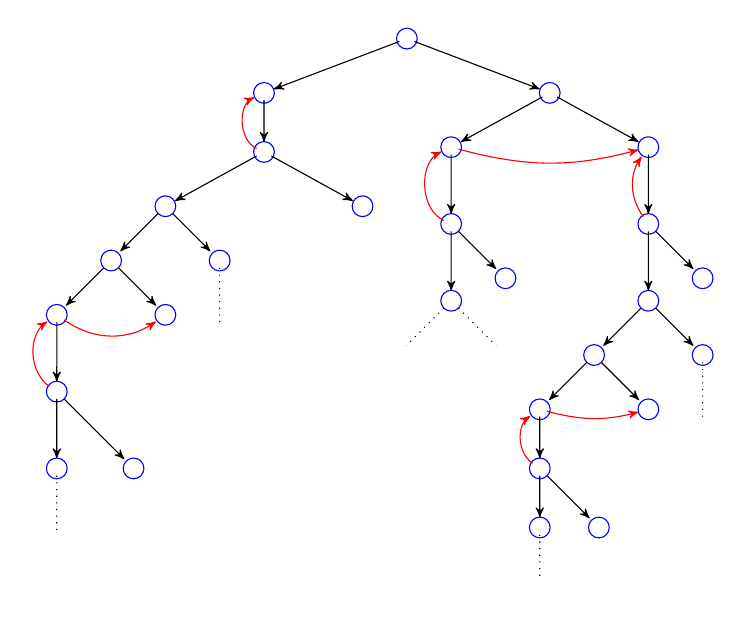
\begin{tikzpicture}[node distance=1.3cm,bend angle=30,transform shape,scale=.75]
		\node(1) {};		
		\node[below right of=1,xshift=1.5cm] (3) {}; 
		\node[below left of=1,xshift=-1.5cm] (22) {};			
		\node[below of=22,node distance=1cm] (221) {};		
		\node[below left of=221,xshift=-.75cm] (5) {};	 
		\node[below right of=221,xshift=.75cm] (222) {};  
		\node[below right of=5] (16) {};		 
		\node[below of=16] (4) {};
		\node[below left of=5] (17) {};
		\node[below left of=17] (18) {}; 
	 \node[below right of=17] (19) {};
	  \node[below of=18] (181) {};
	   \node[below of=181] (182) {};
	   \node[right of=182] (184) {};
	   \node[below of=182] (183) {};
		\node[below right of=3,xshift=.75cm] (6) {};
		\node[below of=6] (61) {};
        \node[below right of=61] (62) {}; 
		\node[below of=61] (51) {};
		\node[below right of=51] (116) {};		 
		\node[below of=116] (41) {};
		\node[below left of=51] (117) {};
		\node[below left of=117] (118) {}; 
	 \node[below right of=117] (119) {};
	  \node[node distance=1cm,below of=118] (1181) {};
	   \node[node distance=1cm,below of=1181] (1182) {};
	  \node[node distance=1cm,below of=1182] (1183) {};
	  \node[node distance=1cm,right of=1182] (1184) {};
	\node[below left of=3,xshift=-.75cm] (31) {};	
	\node[below of=31] (3121) {};
	\node[below of=3121] (312) {};
	\node[below right of=3121] (3122) {};	 
	\node[below right of=312] (311) {};
	\node[below left of=312] (313) {};
	\node[inner sep=0pt,draw, circle, fit=(1184), color=blue] (eqa1) {};
	   \node[inner sep=0pt,draw, circle, fit=(51), color=blue] (eqa1) {};
	   \node[inner sep=0pt,draw, circle, fit=(116), color=blue] (eqa1) {};
	   \node[inner sep=0pt,draw, circle, fit=(117), color=blue] (eqa1) {};
	   \node[inner sep=0pt,draw, circle, fit=(118), color=blue] (eqa1) {};	   
	   \node[inner sep=0pt,draw, circle, fit=(119), color=blue] (eqa1) {};
	   \node[inner sep=0pt,draw, circle, fit=(1181), color=blue] (eqa1) {};
	   \node[inner sep=0pt,draw, circle, fit=(1182), color=blue] (eqa1) {};
	 \node[inner sep=0pt,draw, circle, fit=(1), color=blue] (eq1) {};
     \node[inner sep=0pt,draw, circle, fit=(181), color=blue] (eqf1) {};
     \node[inner sep=0pt,draw, circle, fit=(182), color=blue] (eqa1) {};
     \node[inner sep=0pt,draw, circle, fit=(184), color=blue] (eqa1) {};
	    \node[inner sep=0pt,draw, circle, fit=(22), color=blue] (eq2) {};	    
	    \node[inner sep=0pt,draw, circle, fit=(221), color=blue] (eq2) {};   
	    \node[inner sep=0pt,draw, circle, fit=(222), color=blue] (eq2) {};
	    \node[inner sep=0pt,draw, circle, fit=(3), color=blue] (eq3) {};
	    \node[inner sep=0pt,draw, circle, fit=(5), color=blue] (eq4) {};
	    \node[inner sep=0pt,draw, circle, fit=(16), color=blue] (eq6) {};
	    \node[inner sep=0pt,draw, circle, fit=(19), color=blue] (eq7) {};
	    \node[inner sep=0pt,draw, circle, fit=(18), color=blue] (eq8) {};	
	    \node[inner sep=0pt,draw, circle, fit=(17), color=blue] (eq9) {};
	    \node[inner sep=0pt,draw, circle, fit=(62), color=blue] (eq10) {};  
	    \node[inner sep=0pt,draw, circle, fit=(61), color=blue] (eq10) {};    
	    \node[inner sep=0pt,draw, circle, fit=(6), color=blue] (eq10) {};
	   \node[inner sep=0pt,draw, circle, fit=(3121), color=blue] (eq12) {};
	   \node[inner sep=0pt,draw, circle, fit=(312), color=blue] (eq12) {};
	   \node[inner sep=0pt,draw, circle, fit=(3122), color=blue] (eq12) {};
	   \node[inner sep=0pt,draw, circle, fit=(31), color=blue] (eq13) {};
	   \path[->]
	 	  (18) edge node[above left,pos=0.4] {} (181)
	      (181) edge node[above left,pos=0.4] {} (182)
	      (181) edge node[above left,pos=0.4] {} (184)
	      (1) edge node[above left,pos=0.4] {} (22)
	      (1) edge node[above right,pos=0.4] {} (3)
	      (61) edge node[left,pos=0.4] {} (62)
	      (6) edge node[left,pos=0.4] {} (61)
	      (61) edge node[left,pos=0.4] {} (51)
	      (22) edge node[left,pos=0.4] {} (221)
	      (221) edge node[left,pos=0.4] {} (222)
	      (221) edge node[left,pos=0.4] {} (5)
	      (3) edge node[right,pos=0.4] {} (6)
	      (5) edge node[above left,pos=0.4] {} (16)
	      (5) edge node[above left,pos=0.4] {} (17)
	      (17) edge node[left,pos=0.4] {} (18)
	      (17) edge node[left,pos=0.4] {} (19)
	      (3) edge node[left,pos=0.4] {} (31)
	      (31) edge node[left,pos=0.4] {} (3121)
	      (3121) edge node[left,pos=0.4] {} (3122)
	      (3121) edge node[left,pos=0.4] {} (312)
	      (51) edge node[left,pos=0.4] {} (116)
	      (51) edge node[left,pos=0.4] {} (117)
	      (117)edge node[left,pos=0.4] {} (118)
	      (117)edge node[left,pos=0.4] {} (119)
	      (118)edge node[left,pos=0.4] {} (1181)
	      (1181)edge node[left,pos=0.4] {} (1184)
	      (1181)edge node[left,pos=0.4] {} (1182)
	     ;
	     \path[-,color=black,dotted]
	      (1182)edge node[left,pos=0.4] {} (1183)
	      (16) edge node[left,pos=0.4] {} (4)
	      (182) edge node[above left,pos=0.4] {} (183)
	      (312) edge node[left,pos=0.4] {} (311)
	      (312) edge node[left,pos=0.4] {} (313)
	      (116) edge node[left,pos=0.4] {} (41)
	      ;
	      \path[->,color=red]	         
          (31) edge[bend right=15](6)
	      (118)edge[bend right=15] (119)
	      (61)edge[bend left=35] (6) 
	      (18) edge[bend right=35] (19)	
	      (181) edge[bend left=55] (18)	      
	      (221) edge[bend left=65] (22)
	      (3121) edge[bend left=65](31)
	      (1181)edge[bend left=55] (118) 
	      ;
	     \end{tikzpicture}
	 }
\caption{The -Structure of }
	 \label{fig zpc e}
	\end{figure} 
 

\begin{theorem}\label{theorem-zpc}
 The -Structure associated with  can be computed in  time and space complexity.
\end{theorem}
\begin{proof}
The first step of our Algorithm~\ref{zpc} consists of computing the sets  for all subexpressions  of . 
The set  is represented by an array where the entries are indexed by symbols of . 
The computation of all sets  requires  time and space complexity.\\  

Now that we have computed the sets , the second step consists of the construction of the  Forest. 
Recall that this  Forest encodes the  sets for all subexpressions  of . 
 Therefore, the set  can be obtained by a prefix traversal of the syntax tree of  in  time and space complexity.
\qed
\end{proof}
As each node  encodes  we can state the following lemma.
\begin{lemma}\label{l1}
For a subexpression  of  the set  can be computed in  time and space complexity.
\end{lemma}


For a regular expression , the following algorithm allows to compute the set  for a symbol  and integers .\\

\begin{algorithm}[H]
  \KwIn{Regular Expression .}
  \KwOut{.}
  \nl Calculate~{}\\
      \For{  to  }{
            Compute~\;
       \textbf{end for}}
       Compute~\;
      \Return{}
  \caption{Algorithm for the function  for  and }
  \label{algo:follow}
\end{algorithm}

For each step of the Algorithm~\ref{algo:follow} we will evaluate the complexity in time and in space.


We denote by  the sum of all ranks of symbols 
.\\ 

\noindent\emph{Step~: Computation of }\\
We are interesting about the computation of the sets  and . \\ 


\noindent\emph{Step~: Computation of sets }\\

At each node  of the syntax tree  of , the set  is represented by an array where the entries are indexed by symbols of .
 The computation of the set  requires an  time and space complexity.\\  

\noindent\emph{Step~: Computation of }\\

Now that  for all node , such that , are computed, we can use the techniques outlined in the case of words to calculate the set .  
Indeed, our formulas given in the Proposition~\ref{x} for the computation of  are similar to that defined in the case of words~\cite{Brug,ZPC}. We have the same formulas so we can use the same algorithms used in the paper ~~\cite{ZPC} for the computation of the sets .
Therefore, the computation of   can be done in  time complexity.\\

We denote by  the maximal rank of symbols of  appearing in . Recall that the alphabetic width , of a regular expression  is the sum of occurrences of symbols of a rank greater than  appearing in  that is . The size of the ranked alphabet  is considered as constant. 
\begin{lemma}\label{lemcomplex}
Let  be a regular expression,  be a symbol in  and  be two integers. The sets  for  can be computed in time .
\end{lemma}
As  is bounded by  we can state the following theorem.
\begin{theorem}\label{thmcomplex}
The sets  for all symbols  in  and for all  can be computed with an  time complexity.
\end{theorem}
\subsection{Improving the computation of the function }
In this section we present a simple transformation of the regular expression  which allows us to efficiently compute the sets . For a subexpression  of  and a symbol  in  we associate an expression  obtained from  by replacing the subexpression  by the expression . 
\begin{example}    
For the regular expression . We get  and 
\end{example}
For all subexpressions  of  and for a symbol , the following proposition gives the link between  and .  


\begin{proposition}\label{propFw}
Let  be a regular expression,  be a subexpression of  and  be two integers. 
 
 The set  can be computed as follows: 
 
\end{proposition}
\begin{proof}
\begin{sloppy}  
  
 For a subexpression  of  and from Proposition~\ref{b}, the set  is of the form: 
 where  is the node of  labelled by ,  is the ,  and for  such that . 
 
  
By using this last formula and the modifications: for all symbols  we associate an expression 
 obtained from  by replacing the subexpression  by the expression , then we have for :
 
Therefore, for all symbols : 

\end{sloppy}   
 \qed
\end{proof}

As the rank of the symbol  in  is  and by Lemma~\ref{lemcomplex}, the set  can be computed in time . 
 This step is considered as a preprocessing and is common to each symbol  such that  is in  for all .

So, one can compute in first time the sets  for all  in  in  time complexity. In the second time, from these sets and the set  we construct the set  using  formula of Proposition~\ref{propFw}. This second step can be performed in  time complexity. Indeed from Lemma~\ref{firstComput},  can be computed in time   and the set  can be constructed from the sets computed in the first step with an  time complexity. 

\noindent As  and  and as the first step is performed once for all ,  and for all , then, we can state the following proposition.
\begin{proposition}    
Let  be a regular expression and  be a symbol in . The set  for all  can be computed with an  time complexity. 
\end{proposition}    

Finally we can state the following theorem.

\begin{theorem}
Let  be a regular expression. The computation of the  sets for all symbol  and  can be done with an  time complexity.
\end{theorem}
Our algorithm for the computation of the  sets can be used for the computation of the set of transition rules of the -position automaton, the equation automaton~\cite{automate2,cie}, the -c-continuation automaton~\cite{cie,arxiv} and the Follow automaton~\cite{arxiv}. 
\begin{remark} 
By analogy to the word case, we have chosen to don't consider the constant symbols  in the alphabetic width of . For example for the regular expression , . However, in~\cite{automate2}, the alphabetic width is the number of occurrences of symbols of  in , that is .   
\end{remark}

\section{Conclusion}
In this paper the notion of -position tree automaton associated with the regular
tree expression has been recalled. This automaton is the generalization from words to trees of the position automaton introduced by Glushkov. We give an efficient algorithm that computes the  function from a regular expression  in  time complexity. 

This algorithm for the computation of the  sets can be used for the computation of the set of transitions of the -position, equation, -c-continuation and  automata.  

\bibliographystyle{splncs_srt}
\bibliography{bibliography}
\end{document}
